\chapter{Asymptotic Safety of Gravity-Matter Systems}\label{chap:Matter} 
The calculation in $h^{\mathrm{TT}}$ approximation we performed in the last chapter, already allowed us to investigate the characteristic fixed point structure of the Einstein-Hilbert truncation. Nevertheless, in this part of the thesis, where the impact of minimally coupled matter fields is analyzed, we want to work with the full result, including also the vector and scalar modes arising after the York decomposition (\ref{eqn:York}) of the fluctuation field. 

\section{Inclusion of the other Graviton Modes}
The gauge conditions and the results for the full graviton propagator are taken from \cite{PawlowskiNPgaugeLecture}.\\
For the full solution, we have to take care of an additional gauge fixing term
\begin{equation}
\mathcal{S}_{\mathrm{gf}} = \frac{1}{2\alpha} \int_x \sqrt{\bar{g}} \  \bar{g}^{\mu\nu} F_{\mu}F_{\nu},
\end{equation}
with a gauge fixing parameter $\alpha$ and a De-Donder-type gauge condition given by
\begin{equation}
	F_{\mu} = \bar{\nabla}^{\nu}h_{\mu\nu} - \frac{1+\beta}{4}\bar{\nabla}_{\mu}h^{\nu}_{\phantom{\nu}\nu}. 
\end{equation}
We also have to include a ghost term $\mathcal{S}_{\mathrm{gh}}$ arising from the Faddeev-Popov procedure:
\begin{equation}
\mathcal{S}_{\mathrm{gh}} = Z_c\int_x \sqrt{\bar{g}} \  \bar{g}^{\mu\mu'} \bar{g}^{\nu\nu'}\bar{c}_{\mu'} \mathcal{M}_{\mu\nu}  c_{\nu'}.
\label{eqn:ghost_action}
\end{equation}
 The Faddeev-Popov operator $\mathcal{M}_{\mu\nu}(\bar{g},h)$ reads
\begin{align}
	\mathcal{M}_{\mu\nu} &= \bar{\nabla}^{\rho}(g_{\mu\nu}\nabla_{\rho} + g_{\rho\nu}\nabla_{\mu}) - \bar{\nabla}_{\mu}\nabla_{\nu}.
	\label{eqn:FPop}
\end{align}
If we choose to work in Landau gauge, where $\alpha \equiv 0$ and also set $\beta\equiv 0$, we are able to reduce the dynamical degrees of freedom to two, namely the transverse-traceless mode $h^{\mathrm{TT}}$ and the trace mode $h^{\mathrm{Tr}}$. This choice allows us to simplify the full graviton propagator a lot. We are left with:
\begin{equation} G_{k, h h}=\left(\Gamma^{(2)}_k+R_{k}\right)_{h h}^{-1} = \frac{32\pi}{Z_h}
\begin{pmatrix}
\frac{1}{\bar{\Delta}\left[1+r_{k}\right]-2\Lambda_k+\frac{2}{3}\mathcal{R}} & 0 & 0 & 0 \\[10pt]
0 & 0  & 0 & 0 \\[10pt]
0 & 0 & \frac{-\frac{8}{3}}{\bar{\Delta}\left[1+r_{k}\right]-\frac{4}{3} \Lambda_k}  &0\\[10pt]
0 & 0 & 0 & 0 \\
\end{pmatrix}.
\label{eqn:G_hh}
\end{equation}
For this calculation, the regularized 2-point-function has been determined using a regulator of the form
\begin{equation}
R_{k}=\eval{\Gamma_{k}^{(2)}}_{\bar{R}=0, \Lambda=0} \cdot r_{k}\left(\frac{\bar{\Delta}}{k^2}\right),
\end{equation}
where the shape function $r_k$ is again of Litim-type (\ref{eqn:Litim}). Since we already computed the contributions arising from the $h^{\mathrm{TT}}$ mode in the previous chapter, we only need to compute those from the trace mode $h^{\mathrm{Tr}}$ and the Faddeev-Popov ghosts associated with the graviton sector in the following. 
\vspace{-0.5cm}
\subsection{Trace mode}
For the trace mode $h^{\mathrm{Tr}}$, we take the propagator given in (\ref{eqn:G_hh}):
\begin{equation}
	G_{k, h^{\mathrm{Tr}}h^{\mathrm{Tr}}} =\left(\frac{32\pi}{Z_h}\right) \left(-\frac{8}{3}\right)\frac{1}{\bar{\Delta}\left[1+r_k\right] - \frac{4}{3}\Lambda_k}.
\end{equation}
The respective regulator term reads
\begin{equation}
	R_{k,h^{\mathrm{Tr}}} = -\frac{3}{8}\left(\frac{Z_h}{32\pi}\right)\cdot\bar{\Delta}\cdot r_k\left(\frac{\bar{\Delta}}{k^2}\right).
\end{equation}
We proceed by computing its scale derivative:
\begin{align}
	\partial_t R_{k,h^{\mathrm{Tr}}} = -\frac{3}{8}\left(\frac{Z_h}{32\pi}\right)\cdot\bar{\Delta}\left(\partial_tr_k - \eta_h r_k\right).
\end{align}
In total, the contribution from the r.\,h.\,s. of the flow equation is given by 
\begin{equation}
	\begin{aligned}
	\frac{1}{2}\tr{G_{k, h^{\mathrm{Tr}}h^{\mathrm{Tr}}}\ \partial_t R_{k, h^{\mathrm{Tr}}}} =
		\frac{1}{2}\tr{\frac{\bar{\Delta}\left(\partial_tr_k - \eta_h r_k\right)}{\bar{\Delta}\left[1+r_k\right] - \frac{4}{3}\Lambda_k}}
	\end{aligned}
\end{equation}
To evaluate the functional trace, we make again use of the heat-kernel techniques we already used for the computation in $h^{\mathrm{TT}}$ approximation:

\begin{align}
\frac{1}{2}\tr{\frac{\bar{\Delta}\left(\partial_tr_k - \eta_h r_k\right)}{\bar{\Delta}\left[1+r_k\right] - \frac{4}{3}\Lambda_k}} &= \frac{1}{2} \frac{1}{\left(4 \pi^{2}\right)}\left[\int_{x} \sqrt{\bar{g}}\ \Phi_{2}^{1}\left(-\frac{4}{3}\Lambda_k\right)+\frac{1}{6} \int_{x} \sqrt{\bar{g}} \ \bar{\mathcal{R}} \ \Phi_{1}^{1}\left(-\frac{4}{3}\Lambda_k\right)\right]\nonumber \\
\phantom{.} \\
&= 	\frac{1}{2}\frac{1}{(4\pi)^2}\int_x\sqrt{\bar{g}}\left[ \frac{1}{1-\frac{4}{3}\Lambda_k}\left(\left(1-\frac{\eta_h}{6}\right) + \frac{\bar{\mathcal{R}}}{3}\left(1-\frac{\eta_h}{4}\right)\right)\right].\nonumber
	\end{align}
In the last step, we evaluated the threshold functions using equation (\ref{eqn:threshold}). This already completes the computation of the additional contribution from the trace mode.  
 %TODO: Correct prefactors!!!
 %TODO: Contribution to LHS??
\subsection{Faddeev-Popov ghosts for the graviton sector}
Since we work in a background field approximation, where we assume $g_{\mu\nu}=\bar{g}_{\mu\nu}$, we can simplify the calculations for this part a lot. Nevertheless, we have to be very careful, since we will be confronted with a modified Laplacian, i.\,e. a spin-1 Laplacian $\bar{\Delta}_{\mu\nu}^{'(1)}$, occurring as kinetic operator in the ghost two-point function. A more detailed discussion on how these modified Laplacians effect the values of the heat-kernel coefficients is presented at the end of appendix \ref{chap:AppA}. \\
First we have a look at the Faddeev-Popov operator (\ref{eqn:FPop}). In background field approximation, $\mathcal{M}_{\mu\nu}$ is given by 
\begin{equation}
\begin{aligned}
	\eval{\mathcal{M}_{\mu\nu}}_{g=\bar{g}} &= -\bar{g}_{\mu\nu}\bar{\nabla}^2 + \bar{\nabla}_{\nu}\bar{\nabla}_{\mu} - \bar{\nabla}_{\mu}\bar{\nabla}_{\nu} \\
	&= -\bar{g}_{\mu\nu}\bar{\nabla}^2 - \left[\bar{\nabla}_{\mu}, \bar{\nabla}_{\nu}\right].
\end{aligned}
\end{equation} 
The minus sign in front of the first term arises from integrating by parts to obtain the $\bar{\nabla}^2$ operator. As usual we assumed vanishing boundary terms. Inserting this result into the ghost action (\ref{eqn:ghost_action}) yields
\begin{equation}
	\begin{aligned}
		\mathcal{S}_{\mathrm{gh}} &\overset{\phantom{(\mathrm{\ref{eqn:RiemannB}})}}{=} Z_c\int_x \sqrt{\bar{g}} \ \bar{c}^{\mu}\left[-\bar{g}_{\mu\nu}\bar{\nabla}^2 - \left[\bar{\nabla}_{\mu}, \bar{\nabla}_{\nu}\right]\right]  c^{\nu} \\
		&\overset{(\mathrm{\ref{eqn:RiemannB}})}{=}  Z_c\int_x \sqrt{\bar{g}} \ \bar{c}^{\mu}\underbrace{\left[-\bar{g}_{\mu\nu}\bar{\nabla}^2 - \bar{R}_{\mu\nu}\right]}_{=: \ \bar{\Delta}_{\mu\nu}^{'(1)}} c^{\nu}.
	\end{aligned}
\end{equation}
Note, that the bar referring to the background field should not be confused with the bar in the notation for the conjugated ghost.
We can directly read off the ghost two-point function:
\begin{align}
	\left[\Gamma^{(2)}_{\bar{c}c}\right]_{\mu\nu} = \frac{\delta^2 \mathcal{S}_{\mathrm{gh}}}{\delta c\ \delta\bar{c}} = Z_c \cdot\bar{\Delta}_{\mu\nu}^{'(1)}.
\end{align}
With the following choice of the regulator 
\begin{equation}
	\left[R_{k,c}\right]_{\mu\nu} = Z_c\cdot\bar{\Delta}_{\mu\nu}^{'(1)}\cdot r_k\left(\frac{\bar{\Delta}^{'(1)}}{k^2}\right)
\end{equation}
and its scale derivative
\begin{align}
	\left[\partial_t R_{k,c}\right]_{\mu\nu} =  Z_c\cdot\bar{\Delta}_{\mu\nu}^{'(1)}\left(\partial_tr_k - \eta_c r_k\right),
\end{align}
we arrive at the regularized two-point function for the ghosts: 
\begin{align}
	\left[\Gamma^{(2)}_{k, \bar{c}c}\right]_{\mu\nu} = \left[\Gamma^{(2)}_{\bar{c}c}+ R_{k, c}\right]_{\mu\nu}  = Z_c \cdot\bar{\Delta}_{\mu\nu}^{'(1)}\left(1 + r_k\left(\frac{\bar{\Delta}^{'(1)}}{k^2}\right)\right).
\end{align}
With equation (\ref{eqn:coefficients}), we find the new coefficients for the heat-kernel expansion for the modified Laplacian:
\begin{equation}
\begin{aligned}
	\operatorname{Tr}\mathbf{b}_0\left(\bar{\Delta}^{'(1)}\right) &= 4  \\
	\operatorname{Tr}\mathbf{b}_2\left(\bar{\Delta}^{'(1)}\right) &= \frac{5}{3}\bar{\mathcal{R}}.\\
\end{aligned} 
\end{equation}
All together, we compute the following contribution:
\begin{equation}
\begin{aligned}
	-\tr{G_{k, \bar{c}c}\ \partial_t R_{k,c}} &= -\tr{\frac{\bar{\Delta}_{\mu\nu}^{'(1)}\left(\partial_t r_k - \eta_c r_k\right)}{\bar{\Delta}_{\mu\nu}^{'(1)}\left(1 + r_k\right)}} \\[10pt]
	&=  - \frac{1}{\left(4 \pi^{2}\right)}\left[4\int_{x} \sqrt{\bar{g}}\ \Phi_{2}^{1}\left(0\right)+\frac{5}{3} \int_{x} \sqrt{\bar{g}} \ \bar{\mathcal{R}} \ \Phi_{1}^{1}\left(0\right)\right] \\[10pt]
	&= -\frac{1}{(4\pi)^2}\int_x\sqrt{\bar{g}}\left[4\left(1-\frac{\eta_c}{6}\right) + \frac{10}{3}\bar{\mathcal{R}}\left(1-\frac{\eta_c}{4}\right)\right].
\end{aligned}
\end{equation}
The minus sign in front of the trace is due to the Grassmannian nature of the ghost fields. With the completion of this calculation, we are ready to consider minimally-coupled matter fields.
\section{Matter Contributions in Background Field Approximation}
The inclusion of matter in this theory setting is in principle straightforward. We extend our truncation (\ref{eqn:EHtruncation}) by including an additional matter term: 
\begin{align}
	\Gammak = \Gamma_{\text{EH}} + \mathcal{S}_{\text{gf}}+ \mathcal{S}_{\text{gh}}+ \Gamma_{\text{matter}},
\end{align}
where $\Gamma_{\mathrm{matter}}$ consists of scalar, fermion and gauge field contributions, denoted with $\mathcal{S}_S, \mathcal{S}_D$ and $\mathcal{S}_V$ respectively:
\begin{align}
	\Gamma_{\text{matter}} = \mathcal{S}_S + \mathcal{S}_D + \mathcal{S}_V.
\end{align}
The different actions will be specified later on, every matter type will be treated separately. For conventions regarding the choice of the respective regulators and the general structure of this calculation, we are following \cite{DonaEichhornPercacci2013}. \\
In this truncation we have two essential couplings, $G$ and $\Lambda$ and five inessential\footnote{Inessential in this sense means, that they can be eliminated by field rescalings.} wave function renormalizations $Z_{\Psi}$ with $\Psi = (h,c,S,D,V)$. As before, the wave function renormalizations $Z_{\Psi}$ do not enter the beta functions for $G$ and $\Lambda$ directly, but are still present in a non-trivial way via the anomalous dimension $\eta_{\Psi}$, defined as
\begin{align}
	\eta_{\Psi} = -\partial_t \ln Z_{\Psi}.
\end{align}
For the scalar and gauge field regulators we choose
\begin{align}
	R_{k,\sfrac{S}{V}}(z) = Z_{\sfrac{S}{V}} \cdot \mathbbm{1}_{\sfrac{S}{V}} \cdot \tilde{\Delta}\cdot r_k\left(\frac{\tilde{\Delta}}{k^2}\right),
	\label{eqn:Rk_matter}
\end{align}
where $\tilde{\Delta}= -\nabla^2\mathbbm{1}_{\Psi} + \mathbf{E}_{\Psi}$ is a modified Laplacian, occurring as kinetic operator in the different matter field actions. The Litim-type shape function $r_k$ is in this case the same as the one defined in equation (\ref{eqn:Litim}), now as a function of the modified Laplacian $\tilde{\Delta}$. The regulator choice for the Dirac fermions is slightly different, details are discussed in the respective subsection. Nevertheless, we already present the values of $\mathbf{E}_{\Psi}$ for all three kinetic operators:
\begin{align}
	\mathbf{E}_{\Psi} =  \left\{\begin{array}{ll}{0} & {\text { for } \Psi = S} \\[5pt] {\frac{\mathcal{R}}{4}} & {\text { for } \Psi = D}\\[5pt]  {R^{\mu}_{\phantom{\mu}\nu}} & {\text { for } \Psi = V.}\end{array}\right.
\end{align}
\begin{figure}[t]
	\centering
	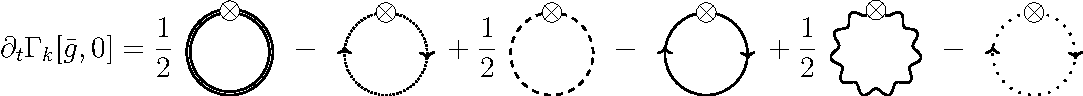
\includegraphics[width=0.95\textwidth]{figs/TikZ/matter_corrections}
\caption[Flow equation for the average effective action $\Gamma_k$ including different matter contributions in diagrammatic representation.]{Flow equation (\ref{eqn:matter_flow}) for the average effective action $\Gamma_k$ including different matter contributions in diagrammatic representation. The double, densely dotted, dashed, solid, wiggly and loosely dotted lines correspond to the graviton, Non-Abelian ghost, scalar, fermion, gauge field  and Abelian ghost propagators, respectively. The crossed circles denote the insertion of the respective regulator.}
	\label{fig:matter_calc}
	\hrulefill
\end{figure}
After having introduced the setup for the following calculation, we are now able to determine the different contributions from the matter fields step by step, by evaluating the functional traces ocurring on the r.\,h.\,s. of the flow equation separately. For the matter configuration in our setting the complete flow equation reads
\begin{equation}
\begin{aligned}
 \partial_t\Gamma_{k} =\frac{1}{2} \operatorname{Tr}&\bigl[G_k\ \partial_t R_{k}\bigr]_{h h} - \operatorname{Tr}\bigl[G_k\ \partial_t R_{k}\bigr]_{\bar{c}c} + \frac{1}{2}\operatorname{Tr}\bigl[G_k\ \partial_t R_{k}\bigr]_{\phi\phi}\\[10pt] -\operatorname{Tr}&\bigl[G_k\ \partial_t R_{k}\bigr]_{\bar{\psi} \psi} 
 +\frac{1}{2}\operatorname{Tr}\bigl[G_k\ \partial_t R_{k}\bigr]_{AA} -\operatorname{Tr}\bigl[G_k\ \partial_t R_{k}\bigr]_{\bar{C}C}\end{aligned}
\label{eqn:matter_flow}
\end{equation}
As before, the minus signs arise due to the fact, that the ghosts and the fermions are Grassmann fields. A digrammatic representation of the flow equation (\ref{eqn:matter_flow}) is depicted in figure (\ref{fig:matter_calc}). \\
For our computation in the background field approximation, we expand the different actions on some background $\bar{g}_{\mu\nu}$ and drop all contributions of $\mathcal{O}(h)$.
\vfill
\subsection{Scalar fields}
The action for $N_S$ scalar fields, minimally coupled to gravity reads
\begin{align}
	\mathcal{S}_S &= \frac{Z_{S}}{2}\int_x \sqrt{g} \ g^{\mu\nu} \ \sum\limits_{i=1}^{N_{\text{S}}} \partial_{\mu}\phi^{i}\partial_{\nu}\phi^{i} \nonumber \\
&=  \frac{Z_{S}}{2}\int_x \sqrt{\bar{g}} \ \bar{g}^{\mu\nu} \ \sum\limits_{i=1}^{N_{\text{S}}} \partial_{\mu}\phi^{i}\partial_{\nu}\phi^{i} + \mathcal{O}(h) \\
&= \frac{Z_{S}}{2}\int_x \sqrt{\bar{g}} \ \ \sum\limits_{i=1}^{N_{\text{S}}} \phi^{i}\left(-\bar{\nabla}^2\right)\phi^{i} + \mathcal{O}(h). \nonumber
\end{align}
In the last step, we use integration by parts and assume vanishing boundary terms. Since $\mathbf{E} =0$ for scalars, we use the initial definition of the Laplacian $\bar{\Delta} = -\bar{\nabla}^2$ for further calculations. These simple manipulations directly allow us to read off the corresponding two-point function
\begin{align}
	\Gamma^{(2)}_{\phi\phi} = \frac{\delta^2 \mathcal{S}_S}{\delta\phi^{i}\ \delta\phi^{j}} = Z_S \cdot\bar{\Delta}\cdot\mathbbm{1}_S + \mathcal{O}(h),
\end{align}
where $\mathbbm{1}_S$ has to be understood as the identity in field space. Using the regulator defined in (\ref{eqn:Rk_matter}), we find the regularized two-point-function:
\begin{align}
	\Gamma^{(2)}_{k, \phi\phi} = \left[\Gamma^{(2)}_{\phi\phi}+ R_{k, S}\right]  = Z_S \cdot\bar{\Delta}\cdot\mathbbm{1}_S\left(1 + r_k\left(\frac{\bar{\Delta}}{k^2}\right)\right).
\end{align}
This expression is already diagonal in field space, meaning we are directly able to invert it to obtain the propagator. Together with the scale derivative of the regulator
\begin{align}
	\partial_t R_{k, S} = Z_S\cdot\mathbbm{1}_S\cdot\bar{\Delta}\left(\partial_t r_k - \eta_S r_k\right),
\end{align}
we can start to evaluate the r.\,h.\,s. of the flow equation:
\begin{equation}
\begin{aligned}
	\frac{1}{2}\tr{G_{k,\phi\phi}\ \partial_t R_{k,S}} &= \frac{1}{2}\tr{\frac{Z_S\cdot\bar{\Delta}\left(\partial_t r_k - \eta_s r_k\right)}{Z_S \cdot\bar{\Delta}\left(1 + r_k\right)}\mathbbm{1}_S}\\[10pt]
	&=   \frac{N_S}{2}\tr{\frac{\bar{\Delta}\left(\partial_t r_k - \eta_s r_k\right)}{\bar{\Delta}\left(1 + r_k\right)}}. 
\end{aligned}
\end{equation}
Here, we already performed the trace operation on the internal indices, leading to an overall factor of $N_S$. The functional trace is again evaluated using heat-kernel techniques. \vfill\newpage
\begin{equation}
\begin{aligned}
	\frac{N_S}{2}\tr{\frac{\bar{\Delta}\left(\partial_t r_k - \eta_s r_k\right)}{\bar{\Delta}\left(1 + r_k\right)}} &= \frac{N_S}{2}\frac{1}{(4\pi^2)}\left[\int_x\sqrt{\bar{g}} \  \Phi_2^1(0) + \frac{1}{6}\int_x\sqrt{\bar{g}} \ \bar{\mathcal{R}}\ \Phi_1^1(0) \right]\\[10pt]
	&= 	\frac{N_S}{2}\frac{1}{(4\pi)^2}\int_x\sqrt{\bar{g}}\left[\left(1-\frac{\eta_S}{6}\right) + \frac{\bar{\mathcal{R}}}{3}\left(1-\frac{\eta_S}{6}\right)\right].
\end{aligned}
\end{equation}
\subsection{Fermionic  fields}
For the fermionic contribution, we  proceed slightly different. First, we present the action for $N_D$ minimally coupled Dirac fermions:
\begin{equation}
	\begin{aligned}
		\mathcal{S}_D &= iZ_D\int_x \sqrt{g} \ \sum\limits_{i=1}^{N_D}\bar{\psi}^{i}\slashed{\nabla}\psi^{i} \\[10pt]
		&=  iZ_D\int_x \sqrt{\bar{g}} \ \sum\limits_{i=1}^{N_D}\bar{\psi}^{i}\bar{\slashed{\nabla}}\psi^{i} + \mathcal{O}(h).
	\end{aligned}
\end{equation}
The Dirac operator $\slashed{\nabla}$ satisfies $\left(i\slashed{\nabla}\right)^2 = -\nabla^2 + \frac{\mathcal{R}}{4} =: \Delta_{\left(\sfrac{1}{2}\right)}$.
Once again, the notation for the conjugated field $\bar{\psi} = \psi^{\dagger}\mathfrak{h}$\footnote{The spin metric $\mathfrak{h}$ satisfies $\abs{\operatorname{det} \mathfrak{h}} = 1$ and $\mathfrak{h}^{-1} = -\mathfrak{h}$.} should not be confused with the bar referring to the background field. As usual, the slashed notation implies contraction with gamma matrices\footnote{In the discussion of Dirac fermions, the gamma matrices $\left\{\gamma^0, \gamma^1, \gamma^2, \gamma^3\right\}$ are a set of complex valued matrices, that constitute an irreducible representation of the Clifford algebra, defined by the anticommutation relation $\left\{\gamma_{\mu}, \gamma_{\nu}\right\}= 2g_{\mu\nu} \mathbbm{1}_{d_{\gamma}\times d_{\gamma}}$, with $d_{\gamma} = 2^{\left[\sfrac{d}{2}\right]}$. A more formal treatment of fermions in curved spacetimes is presented in \cite{LippoldtPHD}.}, i.\,e. $\slashed{\nabla} = \gamma^{\mu}\nabla_{\mu}$.  \\
In principle, this allows us to read off the fermion two-point function
\begin{align}
	\Gamma^{(2)}_{\bar{\psi}\psi} = \frac{\delta^2 \mathcal{S}_D}{\delta \psi^{i}\ \delta \bar{\psi}^{j}} = Z_D\cdot\left(i\bar{\slashed{\nabla}}\right)\cdot\mathbbm{1}_D + \mathcal{O}(h).
\end{align}
For the regularized two-point-function, we choose the following form:
\begin{equation}
\Gamma^{(2)}_{k, \bar{\psi}\psi} = \left[\Gamma^{(2)}_{\bar{\psi}\psi} + R_{k,D}\right] = Z_D\cdot\mathbbm{1}_D\cdot\left(i\bar{\slashed{\nabla}}\right) \left(1+r_{k,D}\left(\frac{ \bar{\Delta}_{\left(\sfrac{1}{2}\right)}}{k^2}\right)\right). \label{eqn:fermion_propagator}
\end{equation}
This allows to determine the expression for $R_{k, D}$ as the difference between the regularized and the initial two-point function:
\begin{equation}
\begin{aligned}
	R_{k,D} &= \Gamma^{(2)}_{k, \bar{\psi}\psi} - \Gamma^{(2)}_{\bar{\psi}\psi} \\[10pt]
	&= Z_D\cdot\left(i\bar{\slashed{\nabla}}\right)\cdot r_{k,D} \cdot\mathbbm{1}_D. \label{eqn:fermion_regulator}
\end{aligned}
\end{equation}
When computing fermion propagators in other theory settings, it follows quite naturally to consider the Dirac dispersion as the \enquote{square root} of the scalar Klein-Gordon dispersion. For a more detailed discussion of this idea in the context of Fermi-Bose mixtures, we refer to chapter 2 of \cite{PawlowskiNPgaugeLecture}. \\
This assumption allows us to express the shape function for the fermions as a function of the scalar shape function:
\begin{align}
\left(1+r_{k,D}\right)^2 = 1+r_{k,S} \qquad \longrightarrow \qquad r_{k, D} = \sqrt{1+r_{k,S}} - 1
\end{align}
Inserting this relation into the expression for the two-point function (\ref{eqn:fermion_propagator}) and the regulator (\ref{eqn:fermion_regulator}), we arrive at:
\begin{equation}
\begin{aligned}
	\Gamma^{(2)}_{k, \bar{\psi}\psi} &=\sqrt{1+r_{k,S}}\cdot Z_D\cdot\left(i\bar{\slashed{\nabla}}\right)\cdot\mathbbm{1}_D \\[10pt] 
	R_{k,D} &= \left(\sqrt{1+r_{k,S}} -1 \right)\cdot Z_D\cdot\left(i\bar{\slashed{\nabla}}\right)\cdot\mathbbm{1}_D.
\end{aligned}
\end{equation}
To invert the Dirac operator $\left(i\slashed{\nabla}\right)$, we use
\begin{equation}
	\left(i\slashed{\nabla}\right)^{-1} =\left(i\slashed{\nabla}\right)^{-1}\cdot\left(\left(i\slashed{\nabla}\right)^{-1}\cdot \ \left(i\slashed{\nabla}\right)\right) = \left(i\slashed{\nabla}\right)\cdot\left(\Delta_{\left(\sfrac{1}{2}\right)}\right)^{-1}
\end{equation}
and therefore the full fermion propagator reads
\begin{equation}
	G_{k, \bar{\psi}\psi} = \frac{\left(i\bar{\slashed{\nabla}}\right)}{Z_D\cdot\bar{\Delta}_{\left(\sfrac{1}{2}\right)}\sqrt{1+r_{k,S}}}\mathbbm{1}_D.
\end{equation}
For the scale derivative of the regulator we find
\begin{equation}
\begin{aligned}
	\partial_tR_{k,D} &=  
	Z_D\cdot\mathbbm{1}_D\left(i\bar{\slashed{\nabla}}\right)\left(\partial_t r_{k,D} - \eta_D r_{k,D}\right) \\[10pt]
	&=Z_D\cdot\mathbbm{1}_D\left(i\bar{\slashed{\nabla}}\right)\left(\frac{\partial_t r_{k,S}}{2\sqrt{1+r_{k, S}}} - \eta_D\left(\sqrt{1+r_{k,S}} -1\right)\right)
\end{aligned} 
\end{equation}
Since we have to deal with the modified spin-$\frac{1}{2}$ Laplacian $\Delta_{\left(\sfrac{1}{2}\right)}$, we have to be careful with the heat-kernel coefficients once again. Using equation (\ref{eqn:coefficients}), we find:
\begin{equation}
\begin{aligned}
	\operatorname{Tr}\mathbf{b}_0\left(\Delta_{\left(\sfrac{1}{2}\right)}\right) &= 4\\
	\operatorname{Tr}\mathbf{b}_2\left(\Delta_{\left(\sfrac{1}{2}\right)}\right) &= \frac{5}{12}\bar{\mathcal{R}}. \\
\end{aligned} 
\end{equation}
All together, we can start to evaluate the r.\,h.\,s. of the flow equation:
\begin{equation}
\begin{aligned}
	-\tr{G_{k, \bar{\psi}\psi}\ \partial_t R_{k,D}} &=-\tr{\frac{Z_D\cdot\bar{\Delta}_{\left(\sfrac{1}{2}\right)}\cdot\left(\frac{\partial_t r_{k,S}}{2\sqrt{1+r_{k, S}}} - \eta_D\left(\sqrt{1+r_{k,S}} -1\right)\right)}{Z_D\cdot\bar{\Delta}_{\left(\sfrac{1}{2}\right)}\sqrt{1 + r_{k,S}}}\mathbbm{1}_D} \\[10pt]
	&= -N_D\tr{\frac{\theta\left(1-\chi\right)}{\chi\left(r_{k,S}(\chi)+1\right)} + \eta_D\left(\frac{1}{\sqrt{r_{k,S}(\chi) + 1}}-1\right)},
	\end{aligned}
\end{equation}
where we substituted $\chi=\frac{\bar{\Delta}_{\left(\sfrac{1}{2}\right)}}{k^2}$. Since we are working with a different shape function, we can not use the definition of the threshold functions this time. Nevertheless, it is still possible, to express this functional trace in terms of the heat kernel expansion. For this explicit trace, we solved the integrals occurring in the associated $Q$-functionals analytically. The most important steps of this calculation can be found in appendix \ref{chap:AppB}. The final contribution after solving all $4$ terms is given by:
\begin{equation}
	-\operatorname{Tr}\left[G_{k, \bar{\psi} \psi} \partial_{t} R_{k, D}\right]= -N_D\frac{1}{(4\pi)^2}\int_x\sqrt{\bar{g}}\left[2\left(1-\frac{\eta_D}{3}\right) + \frac{5}{12}\bar{\Ricci}\left(1-\frac{\eta_D}{2}\right)\right].
\end{equation}
\subsection{Gauge fields}  
The structure of the gauge field contribution is more complex than for the other fields. This is due to the fact, that we have to employ a gauge fixing procedure w.\,r.\,t. the background field $\bar{g}_{\mu\nu}$. This ensures gauge invariance w.\,r.\,t. background gauge transformations. The action for $N_V$ gauge fields, minimally coupled to gravity reads
\begin{equation}
\begin{aligned}
\mathcal{S}_{V} &= \frac{Z_{\text{V}}}{4}\int_x \sqrt{g} \ \sum\limits_{i=1}^{N_{\text{V}}} g^{\mu\nu}g^{\kappa\lambda}F^{i}_{\mu\kappa}F^{i}_{\nu\lambda}  
		+ \frac{Z_{\text{V}}}{2\xi}\int_x \sqrt{\bar{g}} \ \sum\limits_{i=1}^{N_{\text{V}}} \left(\bar{g}^{\mu\nu}\bar{\nabla}_{\mu}A_{\nu}^{i}\right)^2\\
		&+\int_x \sqrt{\bar{g}} \ \sum\limits_{i=1}^{N_{\text{V}}} \bar{C}_i(-\bar{\nabla}^2)C_i, 
\end{aligned}
\end{equation}
where the second term is the gauge fixing term with gauge parameter $\xi$ and the third term is the associated ghost term. Since the two-point function is obtained from a functional derivative w.\,r.\,t. the fields $A^{i}$, we have to evaluate the ghost-term separately. We start by manipulating the first term:
\begin{equation}
\begin{aligned}
\frac{Z_V}{4}\int_x \sqrt{g} \ \sum\limits_{i=1}^{N_{\text{V}}} g^{\mu\nu}g^{\kappa\lambda}F^{i}_{\mu\kappa}F^{i}_{\nu\lambda} &\overset{\phantom{(\mathrm{\ref{eqn:FF2}})}}{=}  \frac{Z_{V}}{4} \int_x \sqrt{\bar{g}} \ \sum\limits_{i=1}^{N_{\text{V}}} \bar{g}^{\mu\nu}\bar{g}^{\kappa\lambda}\bar{F}^{i}_{\mu\kappa}\bar{F}^{i}_{\nu\lambda} + \mathcal{O}(h) \\[5pt]
&\overset{(\mathrm{\ref{eqn:FF2}})}{=} \frac{Z_{V}}{2} \int_x \sqrt{\bar{g}} \ \sum\limits_{i=1}^{N_{\text{V}}} A_{\lambda}^{i}\left[ \bar{\nabla}^{\mu}\bar{\nabla}^{\lambda} - \bar{g}^{\mu\lambda}\bar{\nabla}^2\right]A_{\mu}^{i} + \mathcal{O}(h).
\end{aligned}
\end{equation}
%TODO: Alignment..
The steps we skipped can be found in appendix \ref{chap:AppB}. For the gauge fixing term we find:
\begin{equation}
\begin{aligned}
\frac{Z_{\text{V}}}{2\xi}\int_x \sqrt{\bar{g}} \ \sum\limits_{i=1}^{N_{\text{V}}} \left(\bar{g}^{\mu\nu}\bar{\nabla}_{\mu}A_{\nu}^{i}\right)^2 
	&= \frac{Z_{\text{V}}}{2\xi}\int_x \sqrt{\bar{g}} \ \sum\limits_{i=1}^{N_{\text{V}}} \bar{g}^{\mu\nu}\bar{\nabla}_{\mu}A_{\nu}^{i}g^{\kappa\lambda}\bar{\nabla}_{\kappa}A_{\lambda}^{i} \\[5pt]
	&= \frac{Z_{\text{V}}}{2\xi}\int_x \sqrt{\bar{g}} \ \sum\limits_{i=1}^{N_{\text{V}}} A_{\lambda}^{i}\left[-\bar{\nabla}^{\lambda}\bar{\nabla}^{\mu}\right]A_{\mu}^{i}. 
\end{aligned}	
\end{equation}
In the last step, we integrated by parts and assumed vanishing boundary terms.\\
 This allows us to write 
\begin{equation}
\mathcal{S}_V = \frac{Z_{V}}{2} \int_x \sqrt{\bar{g}} \ \sum\limits_{i=1}^{N_{\text{V}}} A_{\lambda}^{i}\left[ - \bar{g}^{\mu\lambda}\bar{\nabla}^2 +  \bar{\nabla}^{\mu}\bar{\nabla}^{\lambda} - \frac{1}{\xi} \bar{\nabla}^{\lambda}\bar{\nabla}^{\mu}\right]A_{\mu}^{i} \ + \ \text{ghost term}
\end{equation}
In Feynman gauge, where we set $\xi \equiv 1$, this simplifies to
\begin{equation}
\begin{aligned}
\mathcal{S}_V &\overset{\phantom{(\mathrm{\ref{eqn:RiemannB}})}}{=} \frac{Z_{V}}{2} \int_x \sqrt{\bar{g}} \ \sum\limits_{i=1}^{N_{\text{V}}} A_{\lambda}^{i}\left[ - \bar{g}^{\mu\lambda}\bar{\nabla}^2 +  \left[\bar{\nabla}^{\mu}, \bar{\nabla}^{\lambda}\right]\right]A_{\mu}^{i} \ + \ \text{ghost term} \\
&\overset{(\mathrm{\ref{eqn:RiemannB}})}{=} \frac{Z_{V}}{2} \int_x \sqrt{\bar{g}} \ \sum\limits_{i=1}^{N_{\text{V}}} A_{\lambda}^{i}\left[ - \bar{g}^{\mu\lambda}\bar{\nabla}^2 +  \bar{R}^{\mu\lambda}\right]A_{\mu}^{i} \ + \ \text{ghost term}
\end{aligned}
\end{equation}
In this form, we are again directly able to read off the two-point-function:
\begin{equation}
	\left[\Gamma^{(2)}_{AA}\right]^{\mu\nu} = \left[\frac{\delta^2 \mathcal{S}_V}{\delta A^{i}\ \delta A^{j}}\right]^{\mu\nu} = Z_V\underbrace{\left[ - \bar{g}^{\mu\lambda}\bar{\nabla}^2 +  \bar{R}^{\mu\lambda}\right]}_{=: \  \bar{\Delta}^{\mu\nu}_{(1)}}\mathbbm{1}_V + \mathcal{O}(h),
\end{equation} 
where $\bar{\Delta}^{\mu\nu}_{(1)}$ is another a modified spin-one Laplacian, but this time with a different sign in front of the Ricci tensor.  With the respective regulator we find
\begin{align}
	\left[\Gamma^{(2)}_{k, AA}\right]^{\mu\nu} = \left[\Gamma^{(2)}_{AA}+ R_{k, V}\right]^{\mu\nu}  = Z_V \cdot\bar{\Delta}_{(1)}^{\mu\nu}\cdot\mathbbm{1}_V\left(1 + r_k\left(\frac{\bar{\Delta}_{(1)}}{k^2}\right)\right)
\end{align}
and 
\begin{align}
	\left[\partial_t R_{k, V}\right]^{\mu\nu} = Z_V\cdot\bar{\Delta}_{(1)}^{\mu\nu}\cdot\mathbbm{1}_V\left(\partial_t r_k - \eta_V r_k\right).
\end{align}
In this case, the heat-kernel coefficients for $\bar{\Delta}^{\mu\nu}_{(1)}$ read
\begin{equation}
\begin{aligned}
	\operatorname{Tr}\mathbf{b}_0\left(\bar{\Delta}_{(1)}\right) &= 4 \\
	\operatorname{Tr}\mathbf{b}_2\left(\bar{\Delta}_{(1)}\right) &= -\frac{\bar{\mathcal{R}}}{3} \\
\end{aligned} 
\end{equation}
and therefore, the result for the heat-kernel expansion for the gauge fields is given by:

\begin{align}
	\frac{1}{2}\tr{\frac{Z_V\cdot\bar{\Delta}^{\mu\nu}_{(1)}\left(\partial_t r_k - \eta_Vr_k\right)}{Z_V\cdot\bar{\Delta}^{\mu\nu}_{(1)}(1+r_k)}\mathbbm{1}_V} &= \frac{N_V}{2}\tr{\frac{\bar{\Delta}^{\mu\nu}_{(1)}\left(\partial_t r_k - \eta_Vr_k\right)}{\bar{\Delta}^{\mu\nu}_{(1)}(1+r_k)}}\nonumber \\[10pt]
	&= \frac{N_V}{2}\frac{1}{(4\pi)^2}\left[\int_x\sqrt{\bar{g}}\ \Phi_2^1(0) - \frac{1}{3}\int_x\sqrt{\bar{g}}\  \bar{\mathcal{R}} \  \Phi_1^1(0) \right] \\[10pt]
	&=  \frac{N_V}{2}\frac{1}{(4\pi)^2}\int_x\sqrt{\bar{g}}\left[\left(1-\frac{\eta_V}{6}\right)- \frac{2}{3}\bar{\mathcal{R}}\left(1-\frac{\eta_V}{4}\right)\right]\nonumber
\end{align}


To finish the calculation of the gauge field contribution, we need to take the associated ghost term into account. Fortunately, it has already the desired form, where we can directly read off the two-point function:
\begin{equation}
	\Gamma^{(2)}_{\bar{C}C} = \frac{\delta^2 \mathcal{S}_V}{\delta C^{i}\ \delta \bar{C}^{j}} = \mathbbm{1}_V\cdot\bar{\Delta}.
\end{equation} 
Note, that we have the usual Laplacian $\bar{\Delta} = -\bar{\nabla}^2$ as kinetic operator and that no additional wave function renormalization was introduced. The ghost regulator $R_{k, \mathrm{gh}}$ is the same as for the scalar fields and therefore the regularized two-point function reads
\begin{equation}
		\Gamma^{(2)}_{k, \bar{C}C} = \left[\Gamma^{(2)}_{ \bar{C}C}+ R_{k, \mathrm{gh}}\right]  = \bar{\Delta}\cdot\mathbbm{1}_V\left(1 + r_k\left(\frac{\bar{\Delta}}{k^2}\right)\right).
\end{equation} 
In absence of a wave function renormalization, the scale derivative only acts on the shape function $r_k$ and  therefore the final contribution is given by 
\begin{equation}
\begin{aligned}
	-\tr{\frac{\bar{\Delta}\partial_tr_k}{\bar{\Delta}\left(1+r_k\right)}\mathbbm{1}_V} &= -N_{V}\tr{\frac{\bar{\Delta}\partial_tr_k}{\bar{\Delta}\left(1+r_k\right)}} \\[5pt]
	&= -N_V\frac{1}{(4\pi)^2}\left[\int_x\sqrt{\bar{g}} \ \Phi_2^1(0) + \frac{1}{6}\int_x\sqrt{\bar{g}} \bar{\mathcal{R}} \ \Phi_1^1(0) \right] \\[5pt]
	&= -N_V\frac{1}{(4\pi)^2}\int_x\sqrt{\bar{g}}\left[1 + \frac{1}{3}\bar{\mathcal{R}}\right].	
\end{aligned}
\end{equation}  
In the next section, we combine the obtained results and  give the final expressions for the beta functions. 
\section{Beta-Functions and Perturbative Approximation}
We investigate the impact of the different matter fields in a qualitative analysis.  

% \begin{figure}[t]
% \centering
% \hfill
% \begin{subfigure}{0.3\textwidth} 
%	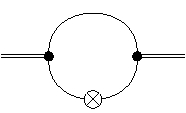
\includegraphics[width=\textwidth]{figs/TikZ/fermion_contribution}
% 	\subcaption{Fermions.}
% \end{subfigure}
% \hfill
% \begin{subfigure}{0.3\textwidth} 
% 	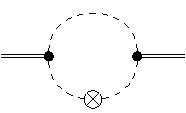
\includegraphics[width=\textwidth]{figs/TikZ/scalar_contribution}
% 	\subcaption{Scalars.}
% \end{subfigure} 
% \hfill
% \begin{subfigure}{0.3\textwidth} 
% 	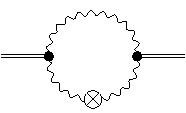
\includegraphics[width=\textwidth]{figs/TikZ/gauge_field_contribution}
% 	\subcaption{Gauge Fields.}
% \end{subfigure} 
% \hfill
% \caption{Different matter contributions to the graviton anomalous dimension $\eta_h$.}	
% \end{figure}
 

 
%  \begin{figure}[t]
% \centering
% \hfill
% \begin{subfigure}{0.3\textwidth} 
%	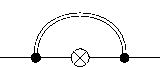
\includegraphics[width=\textwidth]{figs/TikZ/graviton_fluctuations1}
% \end{subfigure}
% \hfill
% \begin{subfigure}{0.3\textwidth}
% \vspace{-3.5pt}
% 	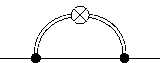
\includegraphics[width=\textwidth]{figs/TikZ/graviton_fluctuations2}
% \end{subfigure} 
% \hfill
% \begin{subfigure}{0.3\textwidth} 
% 	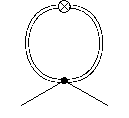
\includegraphics[scale = 1.5]{figs/TikZ/graviton_fluctuations3}
% \end{subfigure} 
% \hfill
% \caption[Contributing diagrams to the fermion anomalous dimension $\eta_D$.]{Contributing diagrams to the fermion anomalous dimension $\eta_D$. Analogous contributions arise for external scalars and gauge fields to $\eta_S$ and $\eta_V$.} 	
% \end{figure}
 
 